\section{Beregninger} \label{Chap:Beregninger}

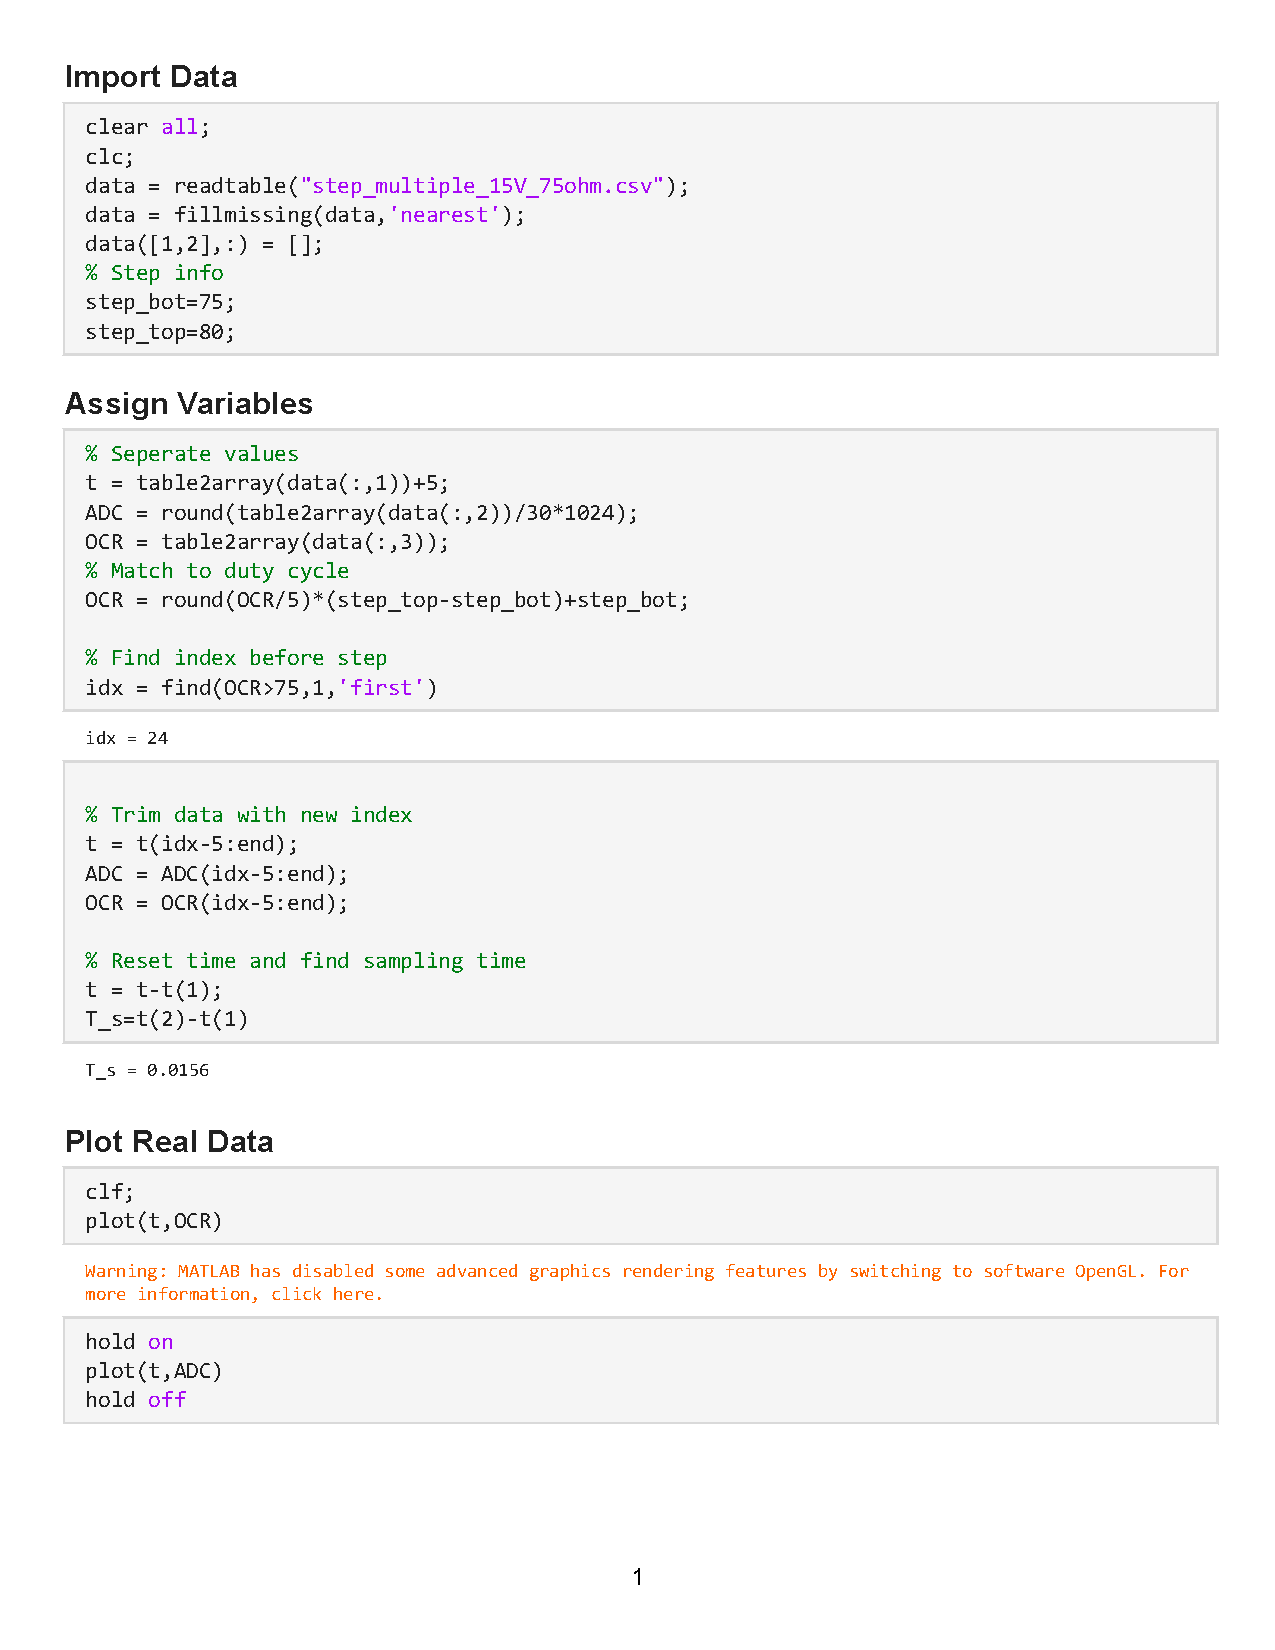
\includepdf[pages=-]{Calculations/PID2.pdf}


\subsection{Transmitterspole/TX-spole}\vspace{5mm}
\underline{Anvendte konstanter}
\begin{align*}
    \mu_0  &= 1.25663706212 \cdot 10^{-6}\: \frac{H}{m}\\
    \rho_{Cu} &= 1.68 \cdot 10^{-8}\: \Omega \cdot m
\end{align*}

\underline{Valgte parametre}
\begin{align*}
    f_r &= 2.00 kHz\\
    r_{spole} &= 13.7cm\\
    A_{pk-pk} &= 8.00V
\end{align*}

\underline{Approksimation af sinusbølgens amplitude}
$$\boxed{a_n=2\cdot\frac{A}{n\cdot\pi}\cdot sin\left(\frac{n\cdot\pi}{2}\right)}$$
\begin{align*}
    a_1 &= 2\cdot\frac{8V}{\pi}\cdot sin\left(\frac{\pi}{2}\right) &= 5.09V\\
    a_{RMS} &= \frac{a_1}{\sqrt{2}} &= 3.60V
\end{align*}
Da kredsløbet udelukkende er resistivt ved resonans:
$$\;\quad R = \frac{a_{RMS}}{I} = \frac{3.60V}{250mA} \;\; \qquad \qquad \qquad = 14.4\Omega$$

\underline{Transmitterspolens antal vindinger}
$$\boxed{N_{TX}=\frac{R \cdot r_{wire}^2}{2 \cdot r_{coil} \cdot \rho}}$$
Ud fra de tilgængelige kobberledninger ($\rho = \rho_{Cu}$), vælges diameteren 0.355mm.
$$N_{TX} = \frac{14.4\Omega\cdot(\frac{0.355mm}{2})^2}{2 \cdot 13.7cm \cdot 1.68 \cdot 10^{-8}\:\Omega\cdot m} = 98.57 \approx 99$$
\underline{Valg af antal lag}\\
For at spolen og dermed spolehovedet ikke skal blive for højt vælges at spolen skal ligge i 5 lag ($n_{lag}=5$)\vspace{5mm}\\
\underline{Vidden af vindingerne (max)}
    $$\boxed{A_{vidde_{max}}= \left\lceil \frac{N_{TX}}{n_{lag}} \right\rceil \cdot d_{wire}}$$
\begin{align*}
    A_{vidde_{max}}&= \left\lceil \frac{99}{5} \right\rceil \cdot 0.355mm &\\
    &= \;\quad 20 \cdot 0.355mm &= 7.10mm
\end{align*}



\underline{Selvinduktans}
$$\boxed{L[\mu H] = \frac{0.394\cdot r_{spole}^2[cm]\cdot N_{TX}^2}{9\cdot r_{spole}[cm]+10\cdot A_{vidde}[cm]}}$$
$$ L_{TX} = \frac{0.394 \cdot 13.7^2 \cdot 99^2}{9 \cdot 13.7 + 10 \cdot 0.710}\mu H = 5.56mH$$
\underline{Kondensatorens kapacitans}
$$\boxed{f_r= \frac{1}{2\cdot\pi\cdot\sqrt{L \cdot C}} \Leftrightarrow C = \frac{1}{4\cdot\pi^2\cdot f_r^2\cdot L}}$$
$$C = \frac{1}{4\cdot \pi^2\cdot 2kHz\cdot 5.56mH} =1.14\mu F$$

\underline{B-felt}
$$\boxed{\lvert \overrightarrow{B} \rvert = \frac{\mu_0\cdot I\cdot N_{TX}}{2\cdot r_{spole}}}$$
$$\lvert \overrightarrow{B} \rvert = \frac{1.26\cdot10^{-6}\frac{H}{m}\cdot250mA\cdot 99}{2\cdot 13.7cm} = 113.5\mu T$$

\subsection{Modtagerspolen (RX)}
Kravspecifikationens pkt. 16 angiver min. 10mH selvinduktans for modtagerspolen.\\
Ved at angive en selvinduktans, der er dobbelt så stor som kravet, opnås en stor fejlmargin ved eventuelle afvigelser mellem teoretiske udregninger og virkelige forhold.
Med udgangspunkt i dette og med antagelsen af at modtagerspolen får samme vidde som transmitterspolen fås følgende:
\begin{align*}
    L_{RX} &= \frac{0.394\cdot 13.7^2\cdot N_{RX}^2}{9\cdot13.7+10\cdot0.71}\mu H & &=20000\mu H\\
           &= \frac{73.98\cdot N_{RX}^2}{130.43} \mu H                            & &=20000\mu H\\
    \lvert N_{RX} \rvert &= 187.8                                                 & &\approx 188
\end{align*}

\subsection{Modtagerspolen (RX)}
\begin{align*}
    L_{RX} &= \frac{0.394\cdot 13.7^2\cdot N_{RX}^2}{9\cdot13.7+10\cdot0.71}\mu H & &=20000\mu H\\
           &= \frac{73.98\cdot N_{RX}^2}{130.43} \mu H                            & &=20000\mu H\\
    \lvert N_{RX} \rvert &= 187.8                                                 & &\approx 188
\end{align*}